\documentclass[12pt]{beamer}
\usepackage[spanish]{babel}
\usepackage[utf8]{inputenc}
\usepackage{xcolor}
\usepackage{listings}
\usepackage{textcomp}
\usepackage{mathpazo}
\usepackage{courier}
\usepackage{fancyvrb}
\usepackage{amsmath}
\usepackage{url}
\usepackage{hyperref}

\newcommand{\onelinerule}{\rule[2.3ex]{0pt}{0pt}}
\newcommand{\twolinerule}{\rule[6.2ex]{0pt}{0pt}}
\newcommand{\respuesta}{\framebox[\textwidth]{\twolinerule}}
\newcommand{\nombre}{%
  \begin{tikzpicture}[xscale=.4,yscale=.7]
    \draw (0, 0) rectangle (22, 1);
  \end{tikzpicture}%
}
%\newcommand{\rol}   {\framebox[0.3\textwidth]{\onelinerule}}
\newcommand{\rol}{%
  \begin{tikzpicture}[xscale=.4,yscale=.7]
    \draw[gray!40] ( 0, 0) grid      ( 9, 1);
    \draw          ( 0, 0) rectangle ( 9, 1);
    \draw          (10, 0) rectangle (11, 1);
    \draw (9 + .2, .5) -- (10 - .2, .5);
  \end{tikzpicture}%
}
\newcommand{\li}{\lstinline}
\providecommand{\pond}[1]{[{\small\textbf{#1\%}}]}

\lstdefinelanguage{py}{%
  classoffset=0,%
    morekeywords={%
      False,class,finally,is,return,None,continue,for,lambda,try,%
      True,def,from,nonlocal,while,and,del,global,not,with,print,%
      as,elif,if,or,yield,assert,else,import,pass,break,except,in,raise},%
    keywordstyle=\color{black!80}\bfseries,%
  classoffset=1,
    morekeywords={int,float,str,abs,len,raw_input,exit,range,min,max,%
      set,dict,tuple,list,bool,complex,round,sum,all,any,zip,map,filter,%
      sorted,reversed,dir,file,frozenset,open,%
      array,zeros,ones,arange,linspace,eye,diag,dot},
    keywordstyle=\color{black!50}\bfseries,%
  classoffset=0,%
  sensitive=true,%
  morecomment=[l]\#,%
  morestring=[b]',%
  morestring=[b]",%
  stringstyle=\em,%
}

\lstdefinelanguage{testcase}{%
  moredelim=[is][\bfseries]{`}{`},%
  backgroundcolor=\color{gray!20},%
}

\lstdefinelanguage{file}{%
  frame=single,%
}

\lstset{language=py}
\lstset{basicstyle=\ttfamily}
\lstset{columns=fixed}
\lstset{upquote=true}
\lstset{showstringspaces=false}
\lstset{rangeprefix=\#\ }
\lstset{includerangemarker=false}

\newlist{certamen}{enumerate}{1}
\setlist[certamen]{%
  label=\arabic*.,
  font=\LARGE\bfseries,%
  labelindent=-.5in,%
  leftmargin=0pt,%
  labelsep=1em%
}



\usecolortheme{seahorse}
\usefonttheme{serif}

\title{Arreglos numéricos}
\author{
  Programación \\ \url{http://progra.usm.cl}
}
\date{}

\begin{document}
  \begin{frame}
    \maketitle
  \end{frame}

  \begin{frame}
    \label{intro-arreglos}
    \frametitle{Arreglos}
    \begin{itemize}
      \item Descargar módulo \li!numpy! \\
        en \url{http://tinyurl.com/bajar-numpy}
        \vfill
      \item Tipo de datos: \li!array!
        \begin{itemize}
          \item colección ordenada de datos,
          \item tamaño fijo,
          \item todos los elementos
            tienen el mismo tipo.
        \end{itemize}
    \end{itemize}
  \end{frame}

  \begin{frame}
    \label{crear-arreglo-valores}
    \frametitle{Crear arreglos usando valores}
    Importar constructor:
    \lstinputlisting[linerange=1-1]{programas/crear-arreglos-valores.py}
    \vfill
    Arreglo de enteros:
    \lstinputlisting[linerange=3-3]{programas/crear-arreglos-valores.py}
    \vfill
    Arreglo de reales:
    \lstinputlisting[linerange=5-6]{programas/crear-arreglos-valores.py}
  \end{frame}

  \begin{frame}
    \label{crear-arreglo-funciones}
    \frametitle{Otras maneras de crear arreglos}
    \lstinputlisting{programas/crear-arreglo-funciones.py}
  \end{frame}

  \begin{frame}
    \label{operaciones-arreglos}
    \frametitle{Operaciones sobre arreglos}
    \lstinputlisting{programas/operaciones-arreglos.py}
  \end{frame}

  \begin{frame}
    \label{comparacion-arreglos}
    \frametitle{Comparación de arreglos}
    \lstinputlisting{programas/arreglos-comparacion.py}
  \end{frame}

  \begin{frame}
    \label{modificar-arreglos}
    \frametitle{Modificar arreglos}
    \footnotesize
    \lstinputlisting{programas/modificar-arreglos.py}
  \end{frame}

  \begin{frame}
    \label{arreglos-aleatorios}
    \frametitle{Arreglos aleatorios}
    \footnotesize
    \lstinputlisting{programas/arreglos-aleatorios.py}
  \end{frame}

  \begin{frame}
    \label{ejercicio-crear-arreglos}
    \frametitle{Ejercicios: creación de arreglos}
    Crear los siguientes arreglos:
    \begin{itemize}
      \item \([5, 5, 5, 5, 5, \ldots, 5, 5, 5, 5, 5]\)\quad(cuarenta elementos)
      \item \([0, 9, 9, 9, 9, \ldots, 9, 9, 9, 9, 0]\)\quad(cien elementos)
      \item \([1, 2, 3, \ldots, 98, 99, 100, 99, 98, \ldots, 3, 2, 1]\)
      \item \([1, 0, 1, 0, 1, 0, 1, 0, 1, 0, 1]\)
      \item \([0, 1, 2, 0, 1, 2, 0, 1, 2, \ldots]\)\quad(tres mil elementos)
      \item Arreglo aleatorio de cien números entre \(-1\) y \(1\)
      \item Arreglo aleatorio de cien números entre \(8.4\) y \(9.7\)
    \end{itemize}
  \end{frame}

  \begin{frame}
    \label{ejercicio-diferencias}
    \frametitle{Ejercicio: diferencias finitas}
    Escriba una función
    que reciba como parámetro un arreglo
    y retorne otro arreglo
    con las diferencias entre elementos consecutivos
    del arreglo original:
    \lstinputlisting{programas/caso-diferencias-arreglo.py}
  \end{frame}

  \begin{frame}
    \label{vectorizacion}
    \frametitle{Aplicación de funciones}
    \lstinputlisting{programas/arreglos-vectorizacion.py}
  \end{frame}

  \begin{frame}
    \label{ejercicio-integral}
    \frametitle{Ejercicio: aproximación de área}
    Calcule el área de la región azul. \\
    La línea roja es el gráfico
    de la función \(y = e^x\).

    \begin{center}
      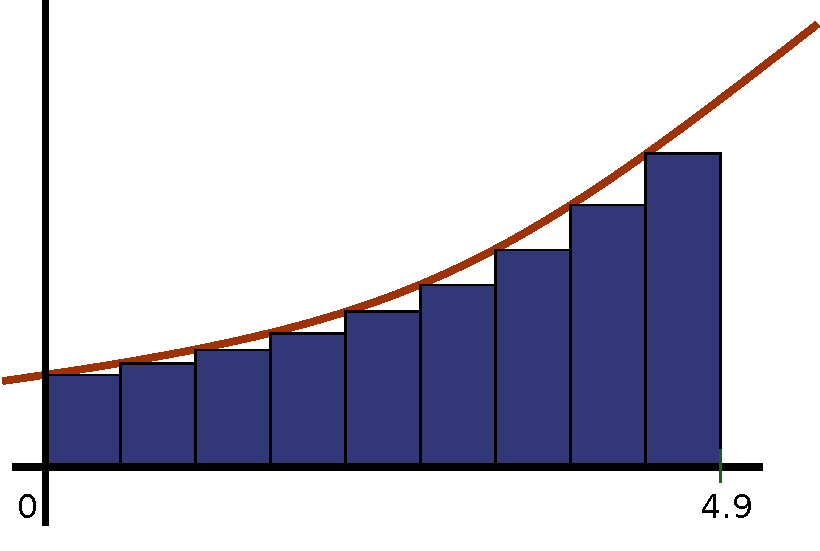
\includegraphics[scale=0.5]{integral}
    \end{center}
  \end{frame}

\end{document}

